\documentclass[a4paper]{article}

\usepackage[english]{babel}
\usepackage[utf8x]{inputenc}
\usepackage{amsmath}
\usepackage{graphicx}
\usepackage[colorinlistoftodos]{todonotes}

\title{Reporte: Actividad 3}

\author{Valenzuela Carrillo María Inés}

\date{20 de Febrero de 2015}

\begin{document}
\maketitle

\section{Fortran}
Como parte de la tercera actividad para el curso de programación se compilaron diversos programas en Fortran. A continuación se describen cada uno de ellos acompañados de un ejemplo del programa en código Fortran y una foto al momento de compilarlos.
\subsection{\underline{ Área }}
En primer programa se pretende calcular el área de un círculo mediante la entrada de un radio.
\subsubsection{Código en Fortran}
\begin{verbatim}
! Area . f90 : Calculates the area of a circle, sample program
! −−−−−−−−−−−−−−−−−−−−−−−−−−−−−−−−−−−−−−−−−−−−−−−
Program area_circulo ! Begin main program
Implicit None ! Declare all variables
Real *8 :: radius , circum , area ! Declare Reals
Real *8 :: PI = 4.0 * atan(1.0) ! Declare , assign Real
Integer :: model_n = 1 ! Declare , assign Ints
print * , 'Enter a radius:' ! Talk to user
read * , radius ! Read into radius
circum = 2.00 * PI * radius ! Calc circumference
area = radius * radius * PI ! Calc area
print * , 'Program number =' , model_n ! Print program number
print * , 'Radius =' , radius ! Print radius
print * , 'Circumference =' , circum ! Print circumference
print * , 'Area =' , area ! Print area
End Program area_circulo ! End main program code
\end{verbatim}

\subsubsection{Captura en la Terminal}
  \begin{center}
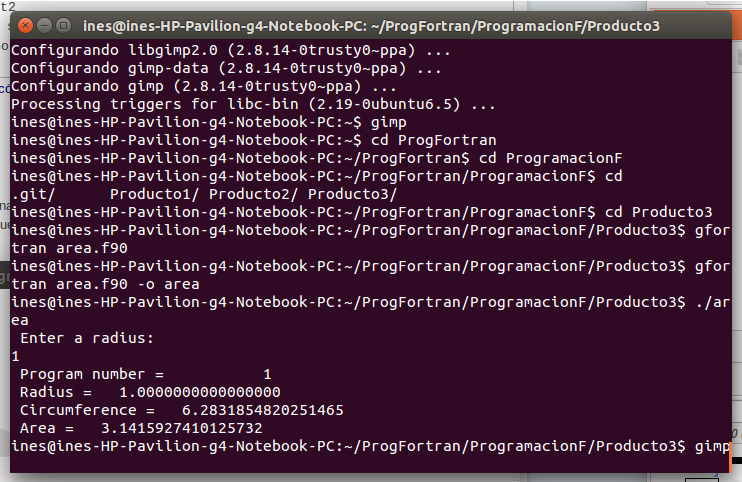
\includegraphics[width=10cm]{area.png}
\end{center}


\subsection{\underline{ Volumen }}
El segundo programa es una modificación del primero, en este caso en lugar de calcular el área se calculará el volumen de una esfera con un líquido dentro, dicho volumen dependerá del radio y de la altura del líquido.

\begin{verbatim}! Volumen . f90 : Calcular el volumen
! −−−−−−−−−−−−−−−−−−−−−−−−−−−−−−−−−−−−−−−−−−−−−−−
Program Volumen_circulo ! Begin main program
  Implicit None ! Declare all variables
  Real *8 :: radius , height , volume ! Declare Reals
  Real *8 :: PI = 4.0 * atan(1.0) ! Declare , assign Real
  Integer :: model_n = 1 ! Declare , assign Ints
  print * , 'Enter a radius:' ! Talk to user
  read * , radius ! Read into radius
  print * , 'Enter a height :' ! Talk to user
  read * , height ! Read into height
  volume = 0.3333 * PI * height * height * (3 * radius - height)  ! Calc volume
  print * , 'Program number =' , model_n ! Print program number
  print * , 'Radius =' , radius ! Print radius
  print * , 'height =' , height ! Print height
  print * , 'volume =' , volume ! Print volume
End Program Volumen_circulo ! End main program code
\end{verbatim}
  
\subsubsection{Captura en la Terminal}
  \begin{center}
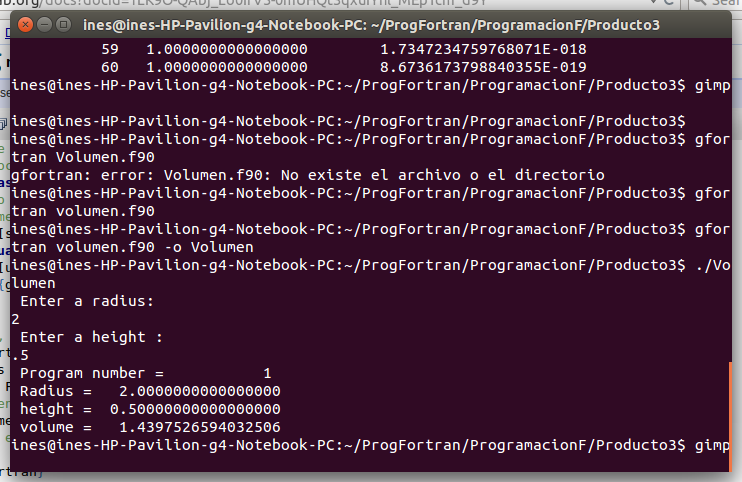
\includegraphics[width=10cm]{volumen.png}
\end{center}
  
\subsection{\underline{Precisión}}
La tercera actividad consistió en determinar la precisión del ordenador, utilizando precisión doble.
  
  \begin{verbatim}
  ! Limits . f90 : Determines machine precision
! −−−−−−−−−−−−−−−−−−−−−−−−−−−−−
Program Limits
  Implicit None
  Integer :: i , n
  Real *8 :: epsilon_m , one
  n=60 ! Establish the number of iterations
  ! Set initial values :
  epsilon_m = 1.0
  one = 1.0
  ! Within a DO−LOOP, calculate each step and print .
  ! This loop will execute 60 times in a row as i is
  ! incremented from 1 to n ( since n = 60) :
  do i = 1, n , 1 ! Begin the do−loop
  epsilon_m = epsilon_m / 2.0 ! Reduce epsilon m
  one = 1.0 + epsilon_m ! Re−calculate one
  print * , i , one , epsilon_m ! Print values so far
   end do ! End loop when i>n
  \end{verbatim}
  
  








\subsubsection{Captura en la Terminal}
  \begin{center}
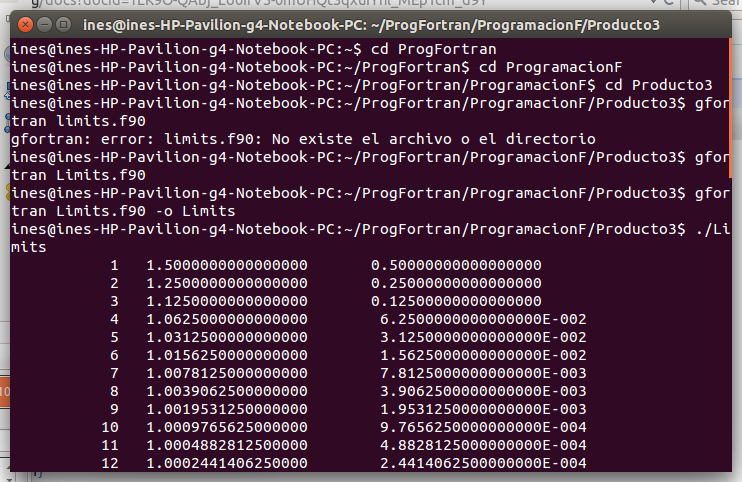
\includegraphics[width=10cm]{Limits.png}
\end{center}
  
  \subsection{\underline{Precisión 4}}
  En esta actividad se hizo lo mismo que en la anterior, pero ahora con precisión sencilla.
  \begin{verbatim}! Limits . f90 : Determines machine precision
! −−−−−−−−−−−−−−−−−−−−−−−−−−−−−
Program Limits
  Implicit None
  Integer :: i , n
  Real *4 :: epsilon_m , one
  n=60 ! Establish the number of iterations
  ! Set initial values :
  epsilon_m = 1.0
  one = 1.0
  ! Within a DO−LOOP, calculate each step and print .
  ! This loop will execute 60 times in a row as i is
  ! incremented from 1 to n ( since n = 60) :
  do i = 1, n , 1 ! Begin the do−loop
  epsilon_m = epsilon_m / 2.0 ! Reduce epsilon m
  one = 1.0 + epsilon_m ! Re−calculate one
  print * , i , one , epsilon_m ! Print values so far
   end do ! End loop when i>n
End Program Limits
  \end{verbatim}
  
 \subsubsection{Captura en la Terminal}
 \begin{center}
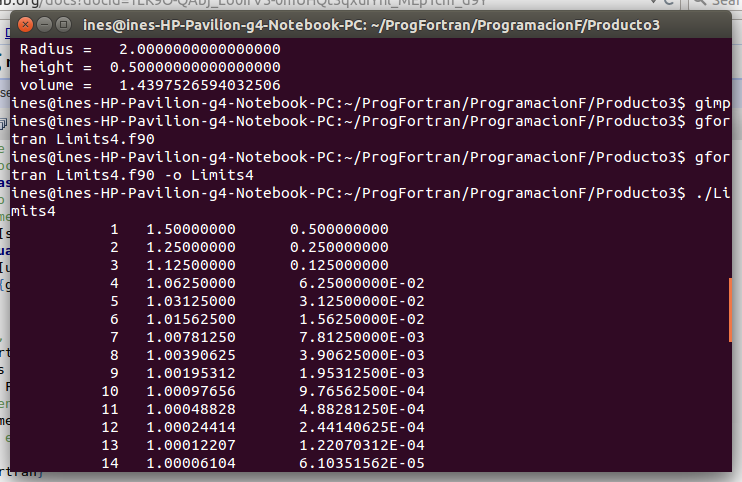
\includegraphics[width=10cm]{Limits4.png}
\end{center}
  
  \subsection{\underline{Math}}
  Se muestran distintas funciones con las cuales se puede trabajar en fortran.








  
    \begin{verbatim}
    ! Math . f90 : demo some Fortran math functions
! −−−−−−−−−−−−−−−−−−−−−−−−−−−−−−−−−−−−−−−−−−
Program Mathtest ! Begin main program
    Real *8 :: x = 1.0 , y, z ! Declare variables x, y, z
    y = sin (x) ! Call the sine function
    z = exp (x) + 1.0 ! Call the exponential function
    print * , x, y, z ! Print x, y, z
End Program Mathtest ! End main program
\end{verbatim}
    
\subsubsection{Captura en la Terminal}
 \begin{center}
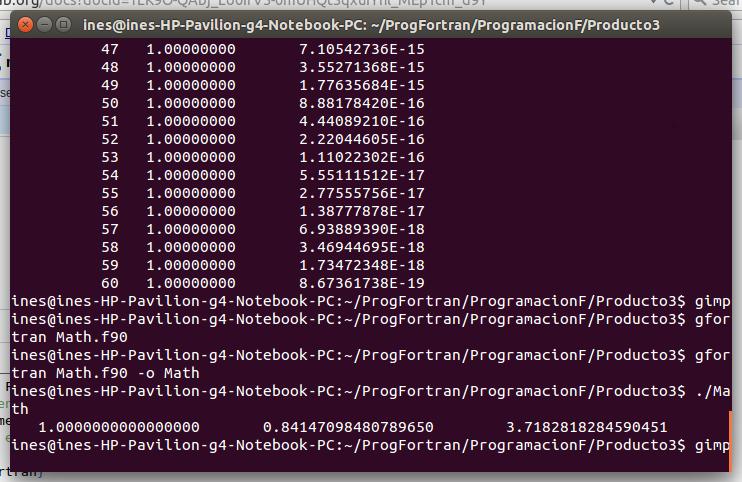
\includegraphics[width=10cm]{Math.png}
\end{center}
    
 \subsection{\underline{Math Complex}}
 
Al igual que en la actividad anterior se muestran funciones, pero que arrojan resultados con números complejos.
  \begin{verbatim}
      ! Math . f90 : demo some Fortran math functions
! −−−−−−−−−−−−−−−−−−−−−−−−−−−−−−−−−−−−−−−−−−
Program Math2! Begin main program
Complex *8 :: x=- 1.0 , y=2, z=0 ! Declare variables x, y, z
x = sqrt (x)
y = asin (y) ! Call the sine function
z = log (z) ! Call the exponential function
print * , x, y, z ! Print x, y, z
End Program Math2 ! End main program
\end{verbatim}
 \subsubsection{Captura en la Terminal}
 \begin{center}
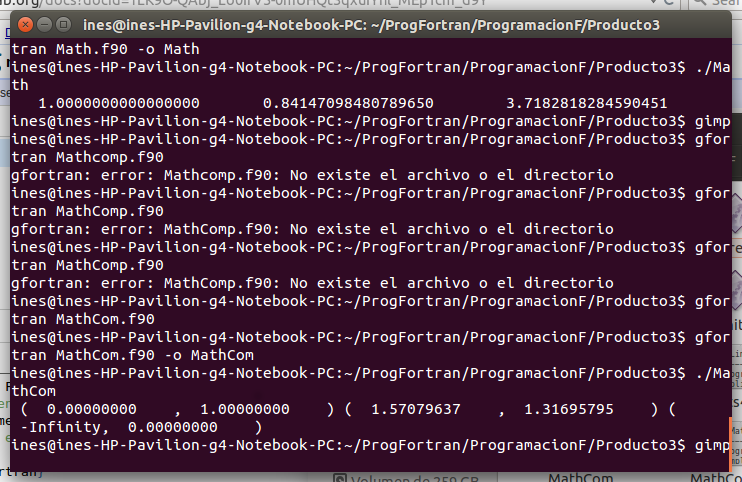
\includegraphics[width=10cm]{MathCom.png}
\end{center}
      
    
\subsection{\underline{función}}
  Se declara una función trigonométrica la cual depende de dos variables dadas por el usuario y se utiliza dicha función en un programa para calcular valores en base a ella.
  
 \begin{verbatim}
        ! Funcion . f90 : Creando funciones
Real *8 Function f (x,y)
  Implicit None
  Real *8 :: x, y
  f = 1.0 + sin (x*y )
End Function f

Program Main
  Implicit None
  Real *8 :: Xin =0.25 , Yin =2. , c , f
  c = f ( Xin , Yin )
  write ( * , * ) 'f(Xin, Yin) = ' , c
End Program Main
    \end{verbatim}
 
\subsubsection{Captura en la Terminal}
 \begin{center}
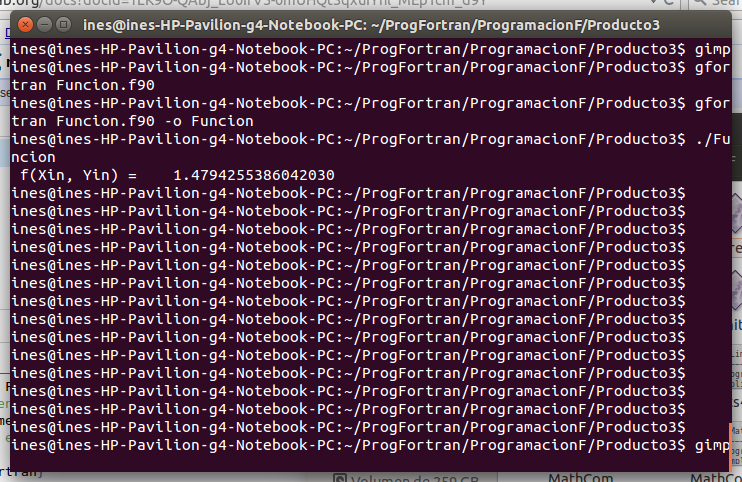
\includegraphics[width=10cm]{Funcion.png}
\end{center}
    
\subsection{\underline{Subroutine}}
  Por último el siguiente código es de subrutinas. Las subrutinas son subprogramas que no devuelven ningún resultado, por tanto no tienen tipo.  
    
\begin{verbatim}
! Subrutina . f90 : Demonstrates the call for a simple subroutine
! −−−−−−−−−−−−−−−−−−−−−−−−−−−−−−−−−−−−−−−−−−−−−
Subroutine g(x, y, ans1 , ans2 )
  Implicit None
  Real (8) :: x , y , ans1 , ans2 ! Declare variables
  ans1 = sin (x*y) + 1.! Use sine intrinsic func.
  ans2 = ans1**2
End Subroutine g
Program Mainprogram ! Demos the CALL
  Implicit None
  Real *8 :: Xin =0.25 , Yin =2.0 , Gout1 , Gout2
  call g( Xin , Yin , Gout1 , Gout2 ) ! Call the subr g
  write ( * , *) 'The answers are: ' , Gout1 , Gout2
End Program Mainprogram
\end{verbatim}
    
\subsubsection{Captura en la Terminal}
 \begin{center}
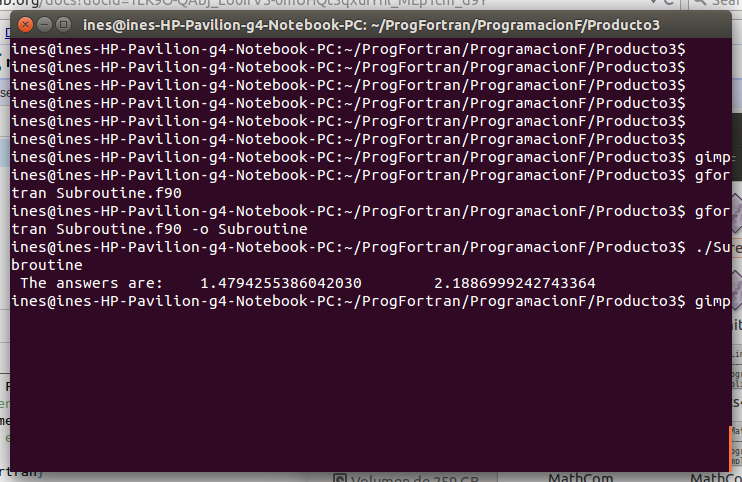
\includegraphics[width=10cm]{Subroutine.png}
\end{center}
\end{document}
